% This file was created with tikzplotlib v0.10.1.
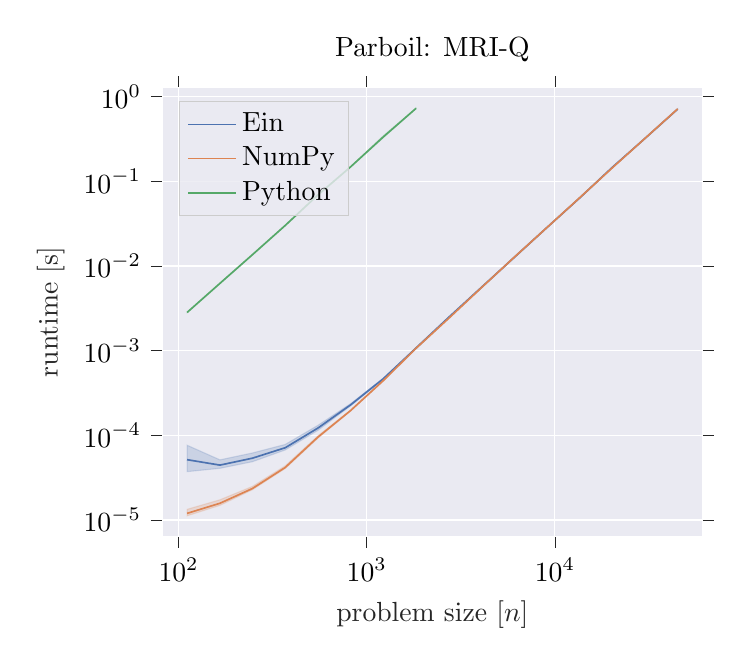
\begin{tikzpicture}

\definecolor{darkslategray38}{RGB}{38,38,38}
\definecolor{lavender234234242}{RGB}{234,234,242}
\definecolor{lightgray204}{RGB}{204,204,204}
\definecolor{mediumseagreen85168104}{RGB}{85,168,104}
\definecolor{peru22113282}{RGB}{221,132,82}
\definecolor{steelblue76114176}{RGB}{76,114,176}

\begin{axis}[
axis background/.style={fill=lavender234234242},
axis line style={white},
legend cell align={left},
legend style={
  fill opacity=0.8,
  draw opacity=1,
  text opacity=1,
  at={(0.03,0.97)},
  anchor=north west,
  draw=lightgray204,
  fill=lavender234234242
},
log basis x={10},
log basis y={10},
tick align=outside,
title={Parboil: MRI-Q},
x grid style={white},
xlabel=\textcolor{darkslategray38}{problem size \(\displaystyle [n]\)},
xmajorgrids,
xmajorticks=true,
xmin=82.2173119053552, xmax=60656.4224057923,
xmode=log,
xtick style={color=darkslategray38},
xtick={1,10,100,1000,10000,100000,1000000},
xticklabels={
  \(\displaystyle {10^{0}}\),
  \(\displaystyle {10^{1}}\),
  \(\displaystyle {10^{2}}\),
  \(\displaystyle {10^{3}}\),
  \(\displaystyle {10^{4}}\),
  \(\displaystyle {10^{5}}\),
  \(\displaystyle {10^{6}}\)
},
y grid style={white},
ylabel=\textcolor{darkslategray38}{runtime \(\displaystyle [\mathrm{s}]\)},
ymajorgrids,
ymajorticks=true,
ymin=6.44509514937527e-06, ymax=1.27001142277489,
ymode=log,
ytick style={color=darkslategray38},
ytick={1e-07,1e-06,1e-05,0.0001,0.001,0.01,0.1,1,10,100},
yticklabels={
  \(\displaystyle {10^{-7}}\),
  \(\displaystyle {10^{-6}}\),
  \(\displaystyle {10^{-5}}\),
  \(\displaystyle {10^{-4}}\),
  \(\displaystyle {10^{-3}}\),
  \(\displaystyle {10^{-2}}\),
  \(\displaystyle {10^{-1}}\),
  \(\displaystyle {10^{0}}\),
  \(\displaystyle {10^{1}}\),
  \(\displaystyle {10^{2}}\)
}
]
\path [draw=steelblue76114176, fill=steelblue76114176, opacity=0.2]
(axis cs:111,7.64748115580005e-05)
--(axis cs:111,3.72972208060673e-05)
--(axis cs:166,4.0835252875695e-05)
--(axis cs:247,4.88473840596271e-05)
--(axis cs:369,6.7268329221406e-05)
--(axis cs:551,0.000114852847618749)
--(axis cs:822,0.000223653940593067)
--(axis cs:1227,0.000462866237739945)
--(axis cs:1830,0.00106242175335865)
--(axis cs:2731,0.00245355305976773)
--(axis cs:4074,0.00557270789158792)
--(axis cs:6078,0.0125523086427165)
--(axis cs:9069,0.0283365872718605)
--(axis cs:13530,0.0632754475533375)
--(axis cs:20185,0.145936900787482)
--(axis cs:30115,0.320605041601812)
--(axis cs:44928,0.712623358200653)
--(axis cs:44928,0.714020192003227)
--(axis cs:44928,0.714020192003227)
--(axis cs:30115,0.321693008599686)
--(axis cs:20185,0.14665374558499)
--(axis cs:13530,0.0637399425110971)
--(axis cs:9069,0.0285860408108601)
--(axis cs:6078,0.0127089362215156)
--(axis cs:4074,0.00564107549882465)
--(axis cs:2731,0.00251207519948366)
--(axis cs:1830,0.00109240443509407)
--(axis cs:1227,0.000473713477222191)
--(axis cs:822,0.000237093156229093)
--(axis cs:551,0.000131444422586355)
--(axis cs:369,7.81547400038107e-05)
--(axis cs:247,6.19402840311523e-05)
--(axis cs:166,5.13782398957119e-05)
--(axis cs:111,7.64748115580005e-05)
--cycle;

\path [draw=peru22113282, fill=peru22113282, opacity=0.2]
(axis cs:111,1.33739018919205e-05)
--(axis cs:111,1.12173942238236e-05)
--(axis cs:166,1.49132007232064e-05)
--(axis cs:247,2.28202668057949e-05)
--(axis cs:369,4.062789333185e-05)
--(axis cs:551,9.28342900732395e-05)
--(axis cs:822,0.000195022538156002)
--(axis cs:1227,0.000440077011060149)
--(axis cs:1830,0.00105853735348736)
--(axis cs:2731,0.00240892100099761)
--(axis cs:4074,0.00553731830009614)
--(axis cs:6078,0.012528845465293)
--(axis cs:9069,0.0282633957795509)
--(axis cs:13530,0.0633936064423404)
--(axis cs:20185,0.143992453522449)
--(axis cs:30115,0.32144269773129)
--(axis cs:44928,0.713192287989754)
--(axis cs:44928,0.720010642417622)
--(axis cs:44928,0.720010642417622)
--(axis cs:30115,0.322048080552488)
--(axis cs:20185,0.144803723048071)
--(axis cs:13530,0.0644441558384659)
--(axis cs:9069,0.0286264725029522)
--(axis cs:6078,0.0128897941919057)
--(axis cs:4074,0.00559594220218362)
--(axis cs:2731,0.00242732959793209)
--(axis cs:1830,0.00108295461147436)
--(axis cs:1227,0.000450903698156903)
--(axis cs:822,0.000199314085446513)
--(axis cs:551,9.87969676543967e-05)
--(axis cs:369,4.36825888719407e-05)
--(axis cs:247,2.49443589484715e-05)
--(axis cs:166,1.73521935363702e-05)
--(axis cs:111,1.33739018919205e-05)
--cycle;

\path [draw=mediumseagreen85168104, fill=mediumseagreen85168104, opacity=0.2]
(axis cs:111,0.00284139199984255)
--(axis cs:111,0.00281315856921844)
--(axis cs:166,0.00620528220835487)
--(axis cs:247,0.0135245814389517)
--(axis cs:369,0.0300064772016471)
--(axis cs:551,0.0690009891442962)
--(axis cs:822,0.148020185515479)
--(axis cs:1227,0.328925585642)
--(axis cs:1830,0.727446436590146)
--(axis cs:1830,0.729701060447134)
--(axis cs:1830,0.729701060447134)
--(axis cs:1227,0.346346094633531)
--(axis cs:822,0.14927478996866)
--(axis cs:551,0.0694211350693412)
--(axis cs:369,0.0302894853075574)
--(axis cs:247,0.0136903077843667)
--(axis cs:166,0.00628679223794377)
--(axis cs:111,0.00284139199984255)
--cycle;

\addplot [semithick, steelblue76114176]
table {%
111 5.16250009241048e-05
166 4.45396020950284e-05
247 5.37770007213112e-05
369 7.14415997208562e-05
551 0.00012215835013194
822 0.000229739699716447
1227 0.000467931201274041
1830 0.00107539789896691
2731 0.00248072924878215
4074 0.00560521049992531
6078 0.0126218833531311
9069 0.0284476669010473
13530 0.0635063490017274
20185 0.146266012140716
30115 0.321243258399772
44928 0.713352350203786
};
\addlegendentry{Ein}
\addplot [semithick, peru22113282]
table {%
111 1.19852447942259e-05
166 1.57818105550113e-05
247 2.35852213674601e-05
369 4.17824449198122e-05
551 9.55665661751828e-05
822 0.000196775694192413
1227 0.000445184290021028
1830 0.00107005975987052
2731 0.00241792426754517
4074 0.00556451805312463
6078 0.0126745723357563
9069 0.0284252734792757
13530 0.0638591521675768
20185 0.144395721890358
30115 0.321745246758947
44928 0.716419132342862
};
\addlegendentry{NumPy}
\addplot [semithick, mediumseagreen85168104]
table {%
111 0.00282732900447953
166 0.00624331846538919
247 0.0136108447615918
369 0.0301533647669631
551 0.0692055784849342
822 0.148659283175515
1227 0.335733234812183
1830 0.728610696513374
};
\addlegendentry{Python}
\end{axis}

\end{tikzpicture}
